\documentclass[10pt]{article}
 
\usepackage[margin=1.5cm]{geometry} 
\usepackage{amsmath,amsthm,amssymb}
\usepackage{polski}
\usepackage[utf8]{inputenc}
\usepackage{siunitx}
\usepackage{graphicx}
\usepackage{comment}
\usepackage[font=scriptsize]{caption}
\usepackage{subcaption} 


 
\newenvironment{theorem}[2][Twierdzenie]{\begin{trivlist}
\item[\hskip \labelsep {\bfseries #1}\hskip \labelsep {\bfseries #2.}]}{\end{trivlist}}
\newenvironment{question}[2][Pytanie]{\begin{trivlist}
\item[\hskip \labelsep {\bfseries #1}\hskip \labelsep {\bfseries #2.}]}{\end{trivlist}}
\newenvironment{hypothesis}[2][Hipoteza]{\begin{trivlist}
\item[\hskip \labelsep {\bfseries #1}\hskip \labelsep {\bfseries #2.}]}{\end{trivlist}}
\newenvironment{lemma}[2][Lemat]{\begin{trivlist}
\item[\hskip \labelsep {\bfseries #1}\hskip \labelsep {\bfseries #2.}]}{\end{trivlist}}
\newenvironment{exercise}[2][Ćwiczenie]{\begin{trivlist}
\item[\hskip \labelsep {\bfseries #1}\hskip \labelsep {\bfseries #2.}]}{\end{trivlist}}
\newenvironment{reflection}[2][Uwaga]{\begin{trivlist}
\item[\hskip \labelsep {\bfseries #1}\hskip \labelsep {\bfseries #2.}]}{\end{trivlist}}
\newenvironment{proposition}[2][Założenie]{\begin{trivlist}
\item[\hskip \labelsep {\bfseries #1}\hskip \labelsep {\bfseries #2.}]}{\end{trivlist}}
\newenvironment{corollary}[2][Wniosek]{\begin{trivlist}
\item[\hskip \labelsep {\bfseries #1}\hskip \labelsep {\bfseries #2.}]}{\end{trivlist}}

\begin{document}

\title{Implementacja population protocols\\oraz testy wydajnościowe}
\author{Grams, Stanisław\\Jezierski, Maciej\\Korczakowski, Juliusz\\ MFI UG\\Algorytmy Numeryczne}

\maketitle
\section {Operacje na macierzach}
\subsection{O implementacji}
Program \textit{„protocols”} został napisany w języku C++, a wyniki działania programu zapisywane są do poszczególnych plików \textit{*.csv}.
\subsection{Zaimplementowane algorytmy}
\begin{itemize}
	\item (PG - Partial Gauss) Algorytm Gaussa z częściowym wyborem elementu
	\item (PGS - Partial Gauss for Sparse Matrices) Algorytm Gaussa z optymalizacją dla macierzy rzadkich
	\item Algroytm Jacobiego
	\item Algorytm Gaussa-Seidela
	\item Metoda Monte Carlo
\end{itemize}

\section{Implementacja i jej poprawność}
\subsection{Generowanie układu równań dla danej liczby agentów}
Generowanie układu równań dla danej liczby agentów $N$ odbywa się w sposób następujący:
\begin{enumerate}
	\item Określenie wszystkich możliwych przypadków (ilość agentów $\#Y$ oraz ilość agentów $\#N$),
	\item Wyliczenie wszystkich możliwych kombinacji bez powtórzeń za pomocą Symbolu Newtona ${{N} \choose {2}}$,
	\item Wygenerowanie równań dla poszczególnych przypadków,
	\item Osadzenie równań w macierzy,
	\item Wypełnienie wektora $B$ zerami.
\end{enumerate}
\subsection{Prawidłowość implementacji}
By zweryfikować poprawność implementacji zarówno generowania macierzy jak i obliczania stworzonego w ten sposób układu równań, wszelkie obliczenia porównywane były z wynikami wyliczonymi metodą Monte Carlo. Poniższy wykres obrazuje dokładność wszystkich zaimplementowanych algorytmów względem metody Monte Carlo na podstawie, którego można wnioskować o poprawności zaimplementowanych metod.

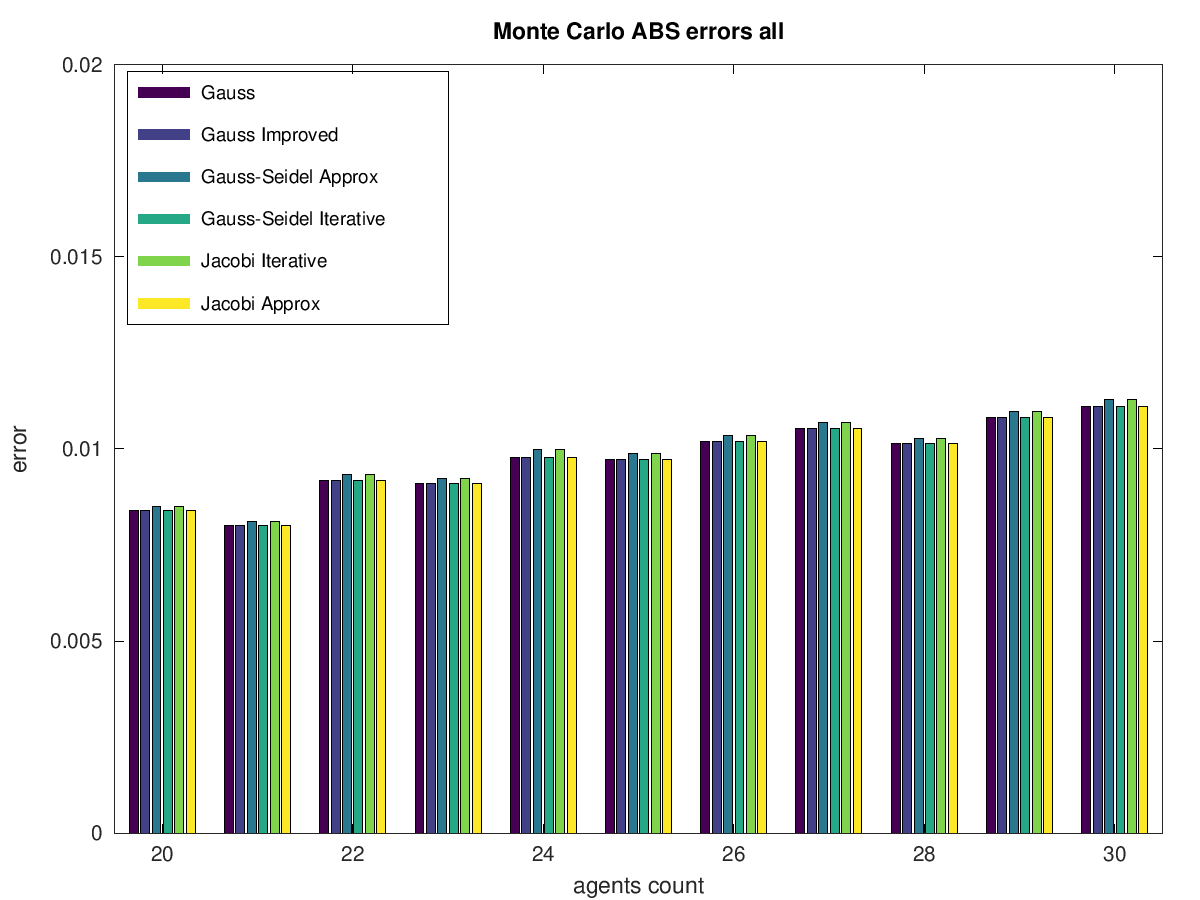
\includegraphics[scale=0.75]{plots/01_abs_all_methods_all_rows.png}

\section{Analiza wyników i wydajność zaimplementowanych algorytmów}

\subsection{Analiza wyników}
\subsubsection{Gauss oraz Gauss z optymalizacją dla macierzy rzadkich}
Przeanalizujmy poniższy wykres. Wynika z niego jednoznacznie, że optymalizacja nie wpływa na dokładność. Wyraźnie widać, że na praktycznie całej długości wykresu błąd wynosi 0.
\begin{figure}[h]
\centering
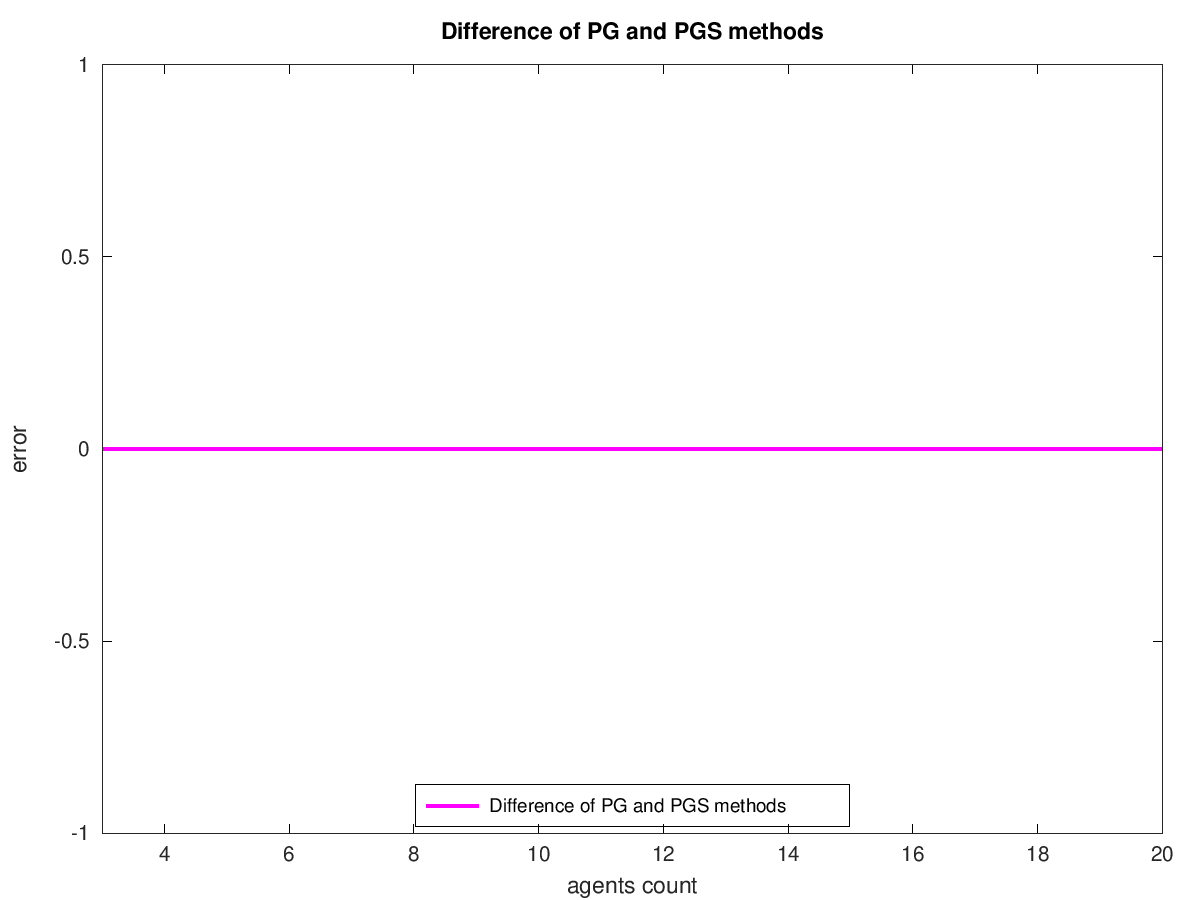
\includegraphics[scale=0.43]{plots/07_abs_gauss_and_gauss_optimized_all_rows.png}
\end{figure}

\subsubsection{Algorytmy iteracyjne}
Obie zaimplementowane przez nasz zespół metody oferują przyzwoitą dokładność jednak poniższe wykresy pozwalają wyciągnąć wniosek mówiący, że metoda Jacobi jest dokładniejsza.

\begin{figure}[h]
\centering
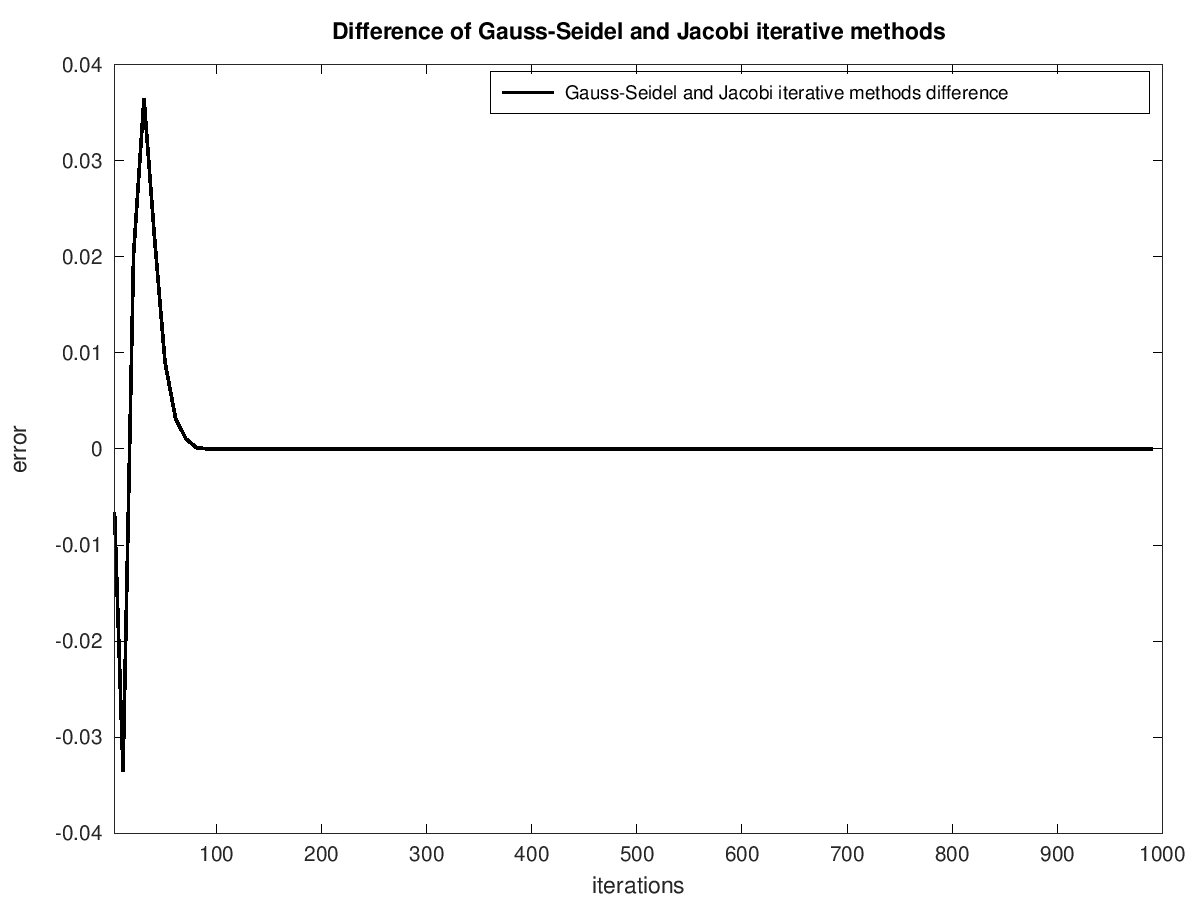
\includegraphics[scale=0.45]{plots/03_abs_iterative_methods_all_rows.png}
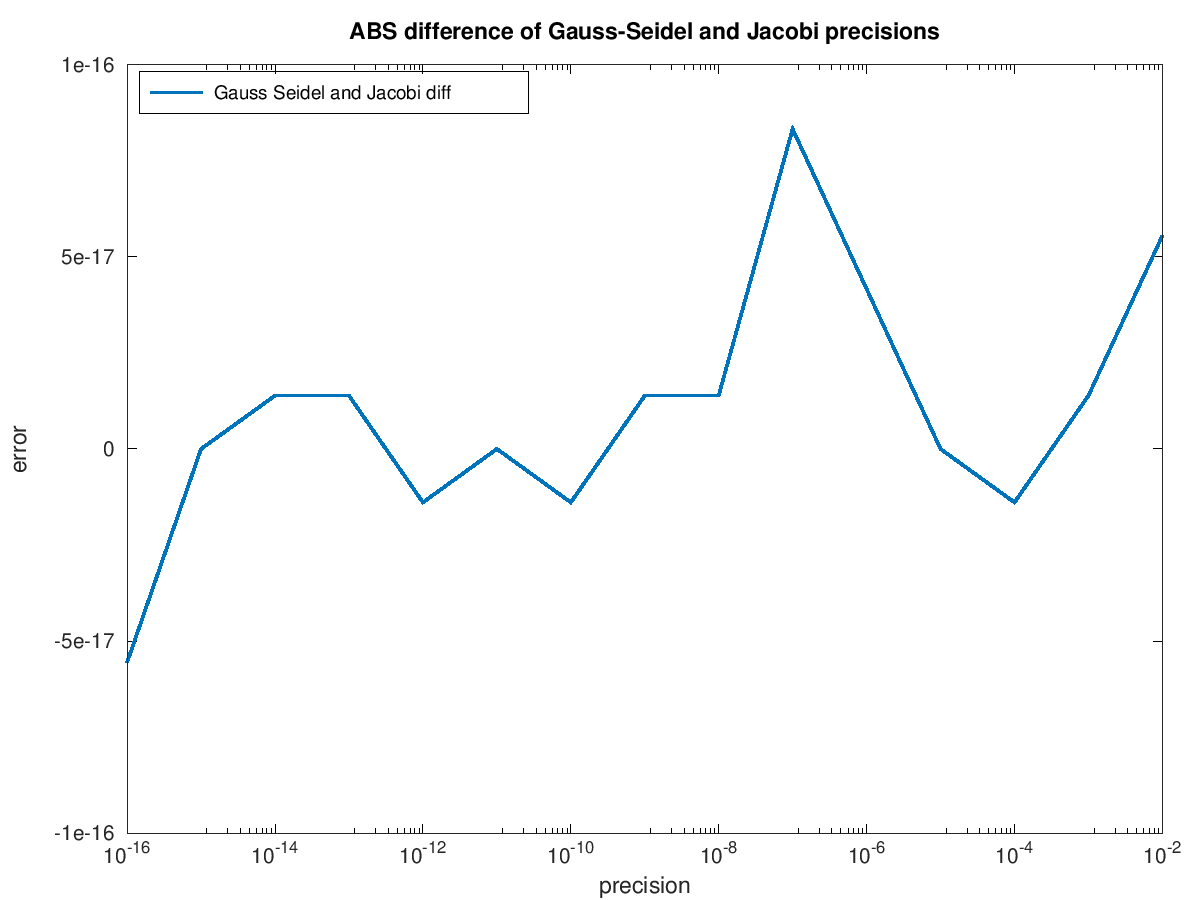
\includegraphics[scale=0.45]{plots/05_abs_precision_methods_all_rows.png}
\end{figure}
\subsection {Wydajność}
\subsubsection{Wydajność względem wielkości planszy}
Analizując poniższe wykresy można wyciągnąć następujące wnioski:\\
1. Pod względem błędów obliczeń metody Gaussa oraz Gaussa z ulepszeniem dla macierzy rzadkich zdecydowanie wygrywają z innymi algorytmami oferując idealnie taką samą, wysoką dokładność.\\
2. Ze względu na swoją specyfikacje metoda Gaussa z ulepszeniem dla macierzy rzadkich wygrywa z klasyczną wersją tej metody pod względem czasu wykonania.\\
\\
Powyższe wnioski wyraźnie wskazują, że w klasie wydajności względem wielkości planszy jako optymalny wybór należy wskazać metodę Gaussa z ulepszeniem dla macierzy rzadkich.
\begin{figure}[h]
\centering
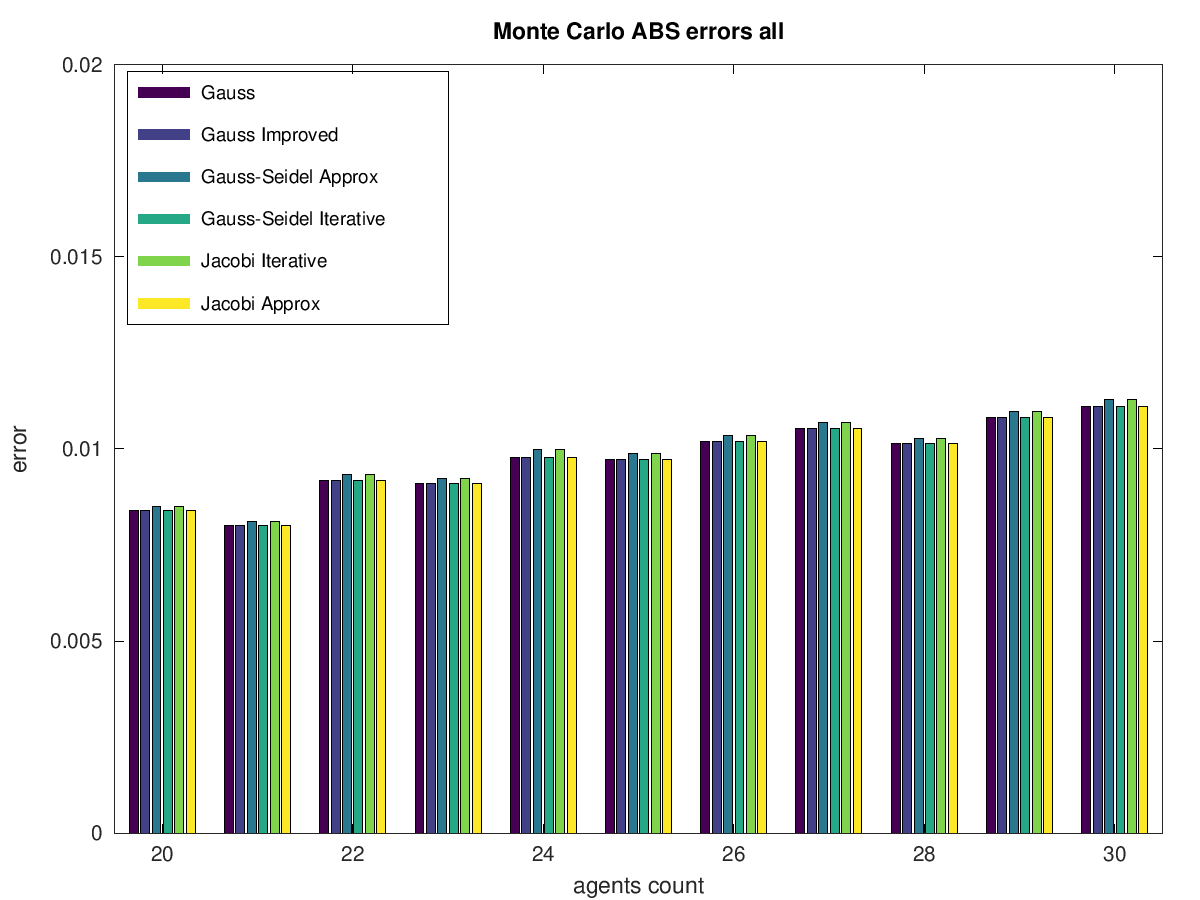
\includegraphics[scale=0.45]{plots/01_abs_all_methods_all_rows.png}
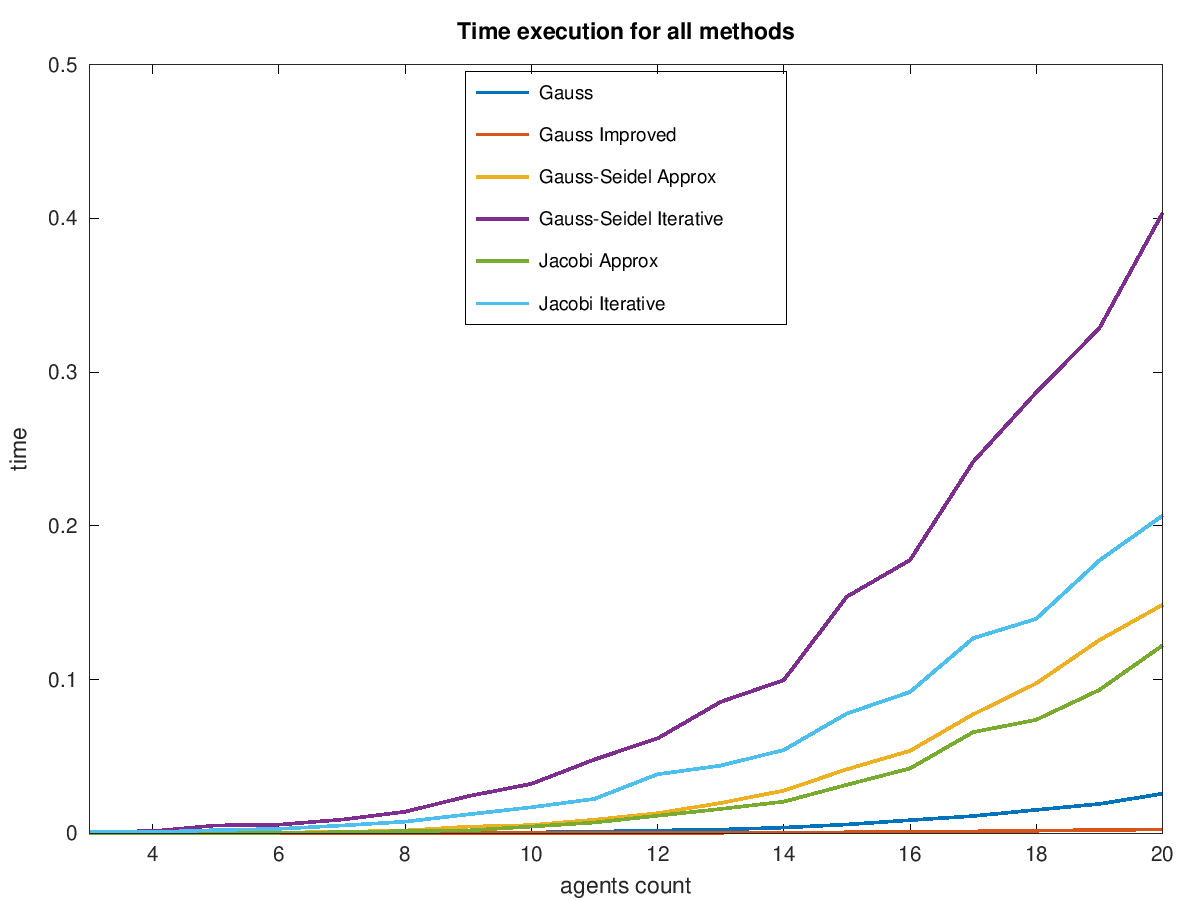
\includegraphics[scale=0.45]{plots/02_time_execution_all_methods.png}
\end{figure}
\newpage

\subsubsection{Wydajność względem zadanej dokładności}
\begin{figure}[h]
\centering
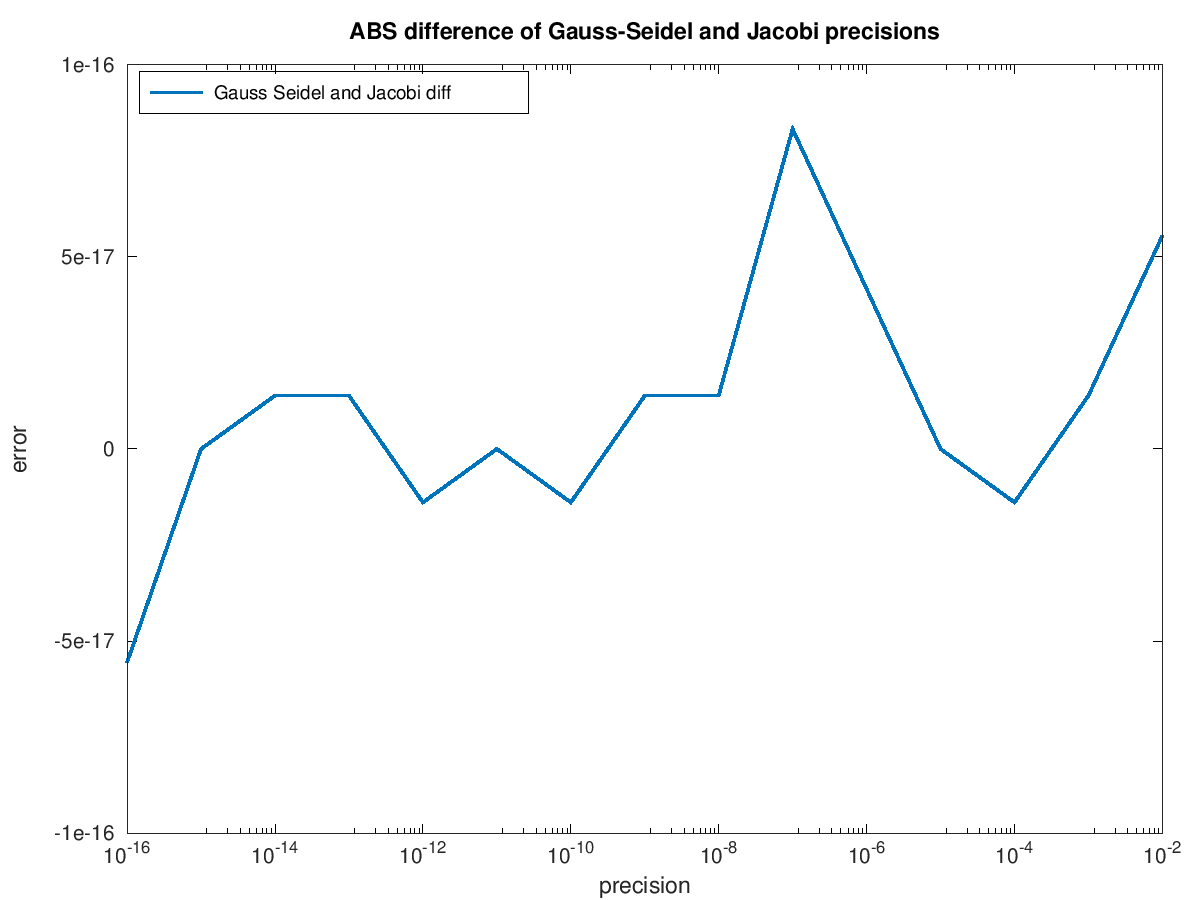
\includegraphics[scale=0.45]{plots/05_abs_precision_methods_all_rows.png}
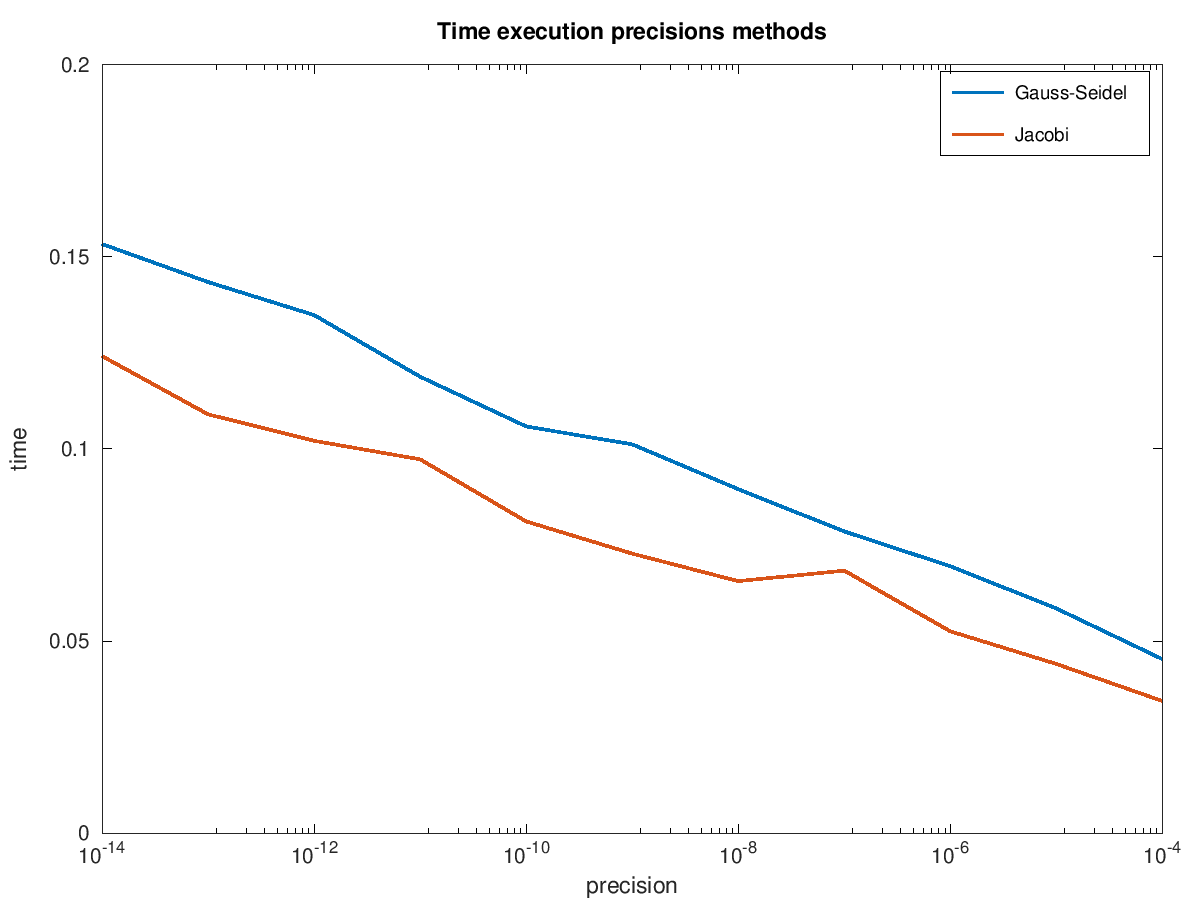
\includegraphics[scale=0.45]{plots/06_time_precision_methods_all_rows.png}
\end{figure}
W przypadku tego kryterium porównujemy tylko metody Jacobiego oraz Gaussa-Seidela. Na pierwszym wykresie widzimy różnicę błędów między powyższymi metodami, w tej kategorii wygrywa metoda Jacobi. W kwestii czasu wykonania oba algorytmy plasują się bardzo podobnie, jednak tak jak w poprzednim przypadku w okolicach $\epsilon$=$10^{-12}$ następuje lekkie załamanie metody Gaussa-Seidela, tym razem na korzyść algorytmu Jacobi.\\
Podsumowując, metoda Jacobi jest dokładniejsza od Gaussa-Seidela, natomiast metoda Gaussa-Seidela jest szybsza od metody Jacobi dla tej samej ilości iteracji.

\section{Podział pracy}
\centering
	\begin{tabular}{| p{5cm} | p{5cm} | p{5cm} |}
		\hline
		\textbf{Stanisław Grams} & \textbf{Juliusz Korczakowski} & \textbf{Maciej Jezierski} \\ \hline
		Implementacja algorytmu Gaussa-Seidela & Implementacja algorytmu Jacobiego & Implementacja algorytmu PG oraz PGS  \\ \hline
		 Implementacja symulacji Monte Carlo& Przygotowanie testów i ich uruchomienie &Analiza wykresów oraz przygotowanie sprawozdania \\ \hline
		Implementacja algorytmu generowania macierzy & Przygotowanie wykresów końcowych &Praca nad strukturą projektu\\ \hline
	\end{tabular}
\end{document}

